%%%%%%%%%%%%%%%%%%%%%%%%%%%%%%%%%%%%%%%%%
%
% (c) 2022 by Jennifer Laaser
%
% This work is licensed under the Creative Commons Attribution-NonCommercial-ShareAlike 4.0 International License. To view a copy of this license, visit http://creativecommons.org/licenses/by-nc-sa/4.0/ or send a letter to Creative Commons, PO Box 1866, Mountain View, CA 94042, USA.
%
% The current source for these materials is accessible on Github: https://github.com/jlaaser/pogil-polymers
%
%%%%%%%%%%%%%%%%%%%%%%%%%%%%%%%%%%%%%%%%%

\renewcommand{\figpath}{content/polymphys/thermal-transitions/Tg/figs}
\renewcommand{\labelbase}{Tg}

\begin{activity}{The Glass Transition}

\begin{instructornotes}
	This activity introduces students to concepts related to glass transitions of polymeric materials.
	
	After completing this activity, students will be able to:
	\begin{enumerate}
		\item Explain the free volume picture of the glass transition, including how the free and occupied volumes of a material change with temperature and why the material eventually hits a point at which the free volume can no longer decrease
		\item Explain how the glass transition temperature of a polymer depends on the polymer's molecular weight
		\item Explain how the glass transition temperature of a polymer depends on the stiffness, sidechain bulkiness or flexibility, and tacticity of the polymer
	\end{enumerate}
	
	\subsection*{Activity summary:}
	\begin{itemize}
		\item \textbf{Activity type:} Learning Cycle
		\item \textbf{Content goals:} See above %Glass Transitions of Polymer Materials
		\item \textbf{Process goals:} %https://pogil.org/uploads/attachments/cj54b5yts006cklx4hh758htf-process-skills-official-pogil-list-2015-original.pdf
			\begin{enumerate}
				\item Interpreting schematics and equations
				\item Linking concepts to derive a key result
				\item Written and oral communication of reasoning
			\end{enumerate}
		\item \textbf{Duration:} 60-75 minutes, including time for class discussion
		\item \textbf{Instructor preparation required:} none beyond knowledge of relevant content
		\item \textbf{Related textbook chapters:}
			\begin{itemize}
				\item \emph{Polymer Chemistry} (Hiemenz \& Lodge), 2nd ed.: sections 12.4 and 12.6
				\item \emph{Introduction to Polymers} (Young \& Lovell), 3rd ed.: sections 16.2 and 16.3
			\end{itemize}
		%\item \textbf{Instructor notes:}
		%	\begin{itemize}
		%		\item \dots
		%	\end{itemize}
	\end{itemize}
	
\end{instructornotes}


\begin{model}[Free Volume]
	\label{\labelbase:mdl:freevolume}
	
	The following cartoon depicts the changes that happen at the molecular level as a polymer is cooled from high temperature to low temperature:
	
	\centerline{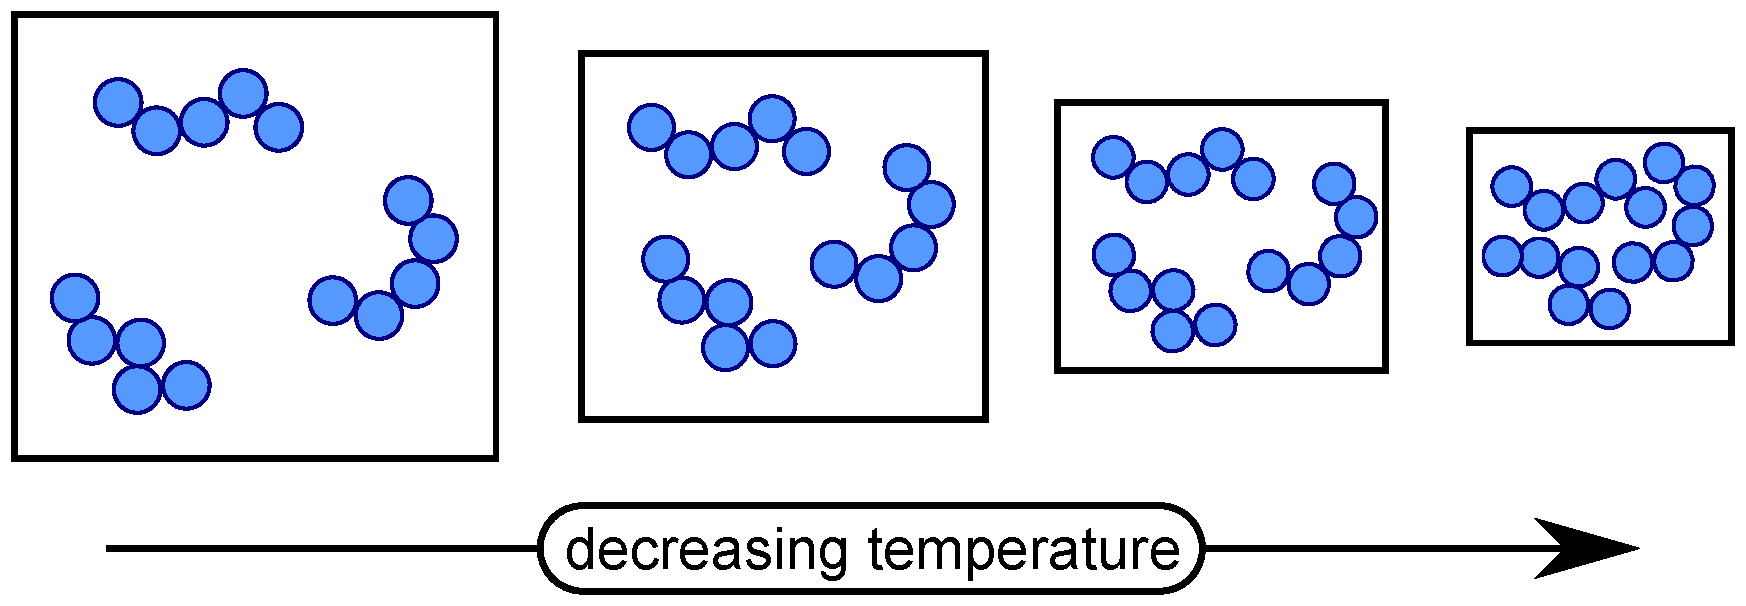
\includegraphics[width=0.65\textwidth]{\figpath/Model1_FreeVolume}}
	
	In this image, the shaded circles represent the \textit{occupied volume} of the polymers, which reflects their van der Waals radii plus the space required for their chemical bonds to vibrate.  The white area represents the \emph{free volume} of the material, which is the space available for the polymer chains to rotate and translate.
	
\end{model}


\begin{ctqs}

	\question Briefly indicate how each of the following changes as the temperature of the sample is lowered:
	
		\begin{enumerate}
		
			\item the occupied volume:
			
				\begin{solution}[0.25in]{}
					The occupied volume decreases (the size of the blue circles gets smaller)
				\end{solution}
			
			\item the free volume:
			
				\begin{solution}[0.25in]{}
					The free volume decreases (the amount of white space in the box gets smaller)
				\end{solution}
			
			\item the overall density of the material:
			
				\begin{solution}[0.25in]{}
					The density increases (the same amount of material is packed into a smaller volume)
				\end{solution}
			
		\end{enumerate}
		
	\question On the following axes, sketch lines depicting how the total volume, $V_{tot}$, and the occupied volume, $V_{occ}$, change with temperature.  Then, \emph{shade in} the area on the plot that corresponds to the free volume, $V_f$. \label{\labelbase:ctq:VTplot1}
	
		\vspace{0.25in}
		\begin{solution}[1.5in]{
			\centerline{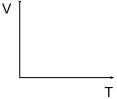
\includegraphics[width=0.33\textwidth]{\figpath/Model1_VTaxes}}
		}
			\centerline{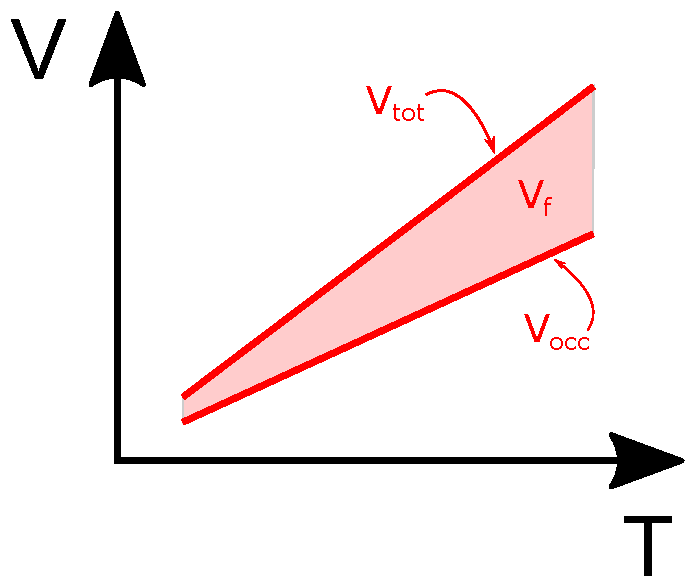
\includegraphics[width=0.33\textwidth]{\figpath/Model1_VTaxes_ctq2}}
		\end{solution}
		
	\question As the free volume decreases, it takes more and more time for the polymer chains to rearrange.  How do you expect this to affect... \label{\labelbase:ctq:viscosityconcept}
	
		\begin{enumerate}
			\item ... the relaxation time of the material?
			
				\begin{solution}[0.5in]{}
					As the free volume decreases, the relaxation time of the material should increase because it takes more time for the polymer chains to rearrange.
				\end{solution}
			
			\item ... the viscosity of the material?
			
				\begin{solution}[0.5in]{}
					As the free volume decreases, the viscosity of the material should increase because it is harder for the chains to rearrange and flow.
				\end{solution}
				
		\end{enumerate}
	
\end{ctqs}

\begin{infobox}

	The viscosity of polymer melts can be described by
	\begin{equation*}
		\eta = A' e^{\frac{B' V_{occ}}{V_f}}
	\end{equation*}
	where $A'$ and $B'$ are positive constants.  With some rearrangement, and the assumption that the fraction of the material that is free volume increases linearly with temperature, this expression can be rewritten
	\begin{equation*}
		\eta = A e^{\frac{B}{T-T_0}}
	\end{equation*}
	where $T_0$ is the \emph{Vogel temperature}.  This expression is known as the \emph{Vogel-Fulcher-Tamman} (or VFT) \emph{equation}.
			
\end{infobox}

\begin{ctqs}
		
	\question Are these expressions consistent with the pictures shown in Model \ref{\labelbase:mdl:freevolume} and the trend you predicted in CTQ \ref{\labelbase:ctq:viscosityconcept}?  Briefly explain your group's reasoning.
			
				\begin{solution}[2in]{}
					Yes.  Students may look at this a couple of different ways:
					
					First, as shown in the model, the free volume decreases much more quickly than the occupied volume, so $V_{occ}/V_f$ gets big as the free volume decreases.  Since this term is in the exponent in the first equation for $\eta$, the exponential term (and thus the viscosity) also gets larger as the free volume increases, consistent with the prediction from the previous question.
					
					Second, if students prefer to think about the temperature dependence, they will note that as $T$ decreases toward the Vogel temperature, the denominator in the exponent becomes small ($T-T_0\to 0$), so the exponent again becomes large ($B/(T-T_0) \to \infty$).  This again means that the viscosity increases significantly as the temperature (and free volume) decrease toward $T_0$.
				\end{solution}
	
	\clearpage
	\question At some temperature, the relaxation time of the material will become so slow that the polymers are effectively unable to keep rearranging to find higher-density/lower free-volume configurations.  After this point, further decreases in the temperature will not significantly change the free volume of the polymer. \label{\labelbase:ctq:traptemp}
	
		Based on this information, propose a revised version of your plot from CTQ \ref{\labelbase:ctq:VTplot1} that more accurately depicts the temperature dependence of the free volume and the total volume of a real polymer material.  Make sure the transition temperature is clearly labeled.
	
		\vspace{0.25in}
	
		\begin{solution}[1.5in]{
			\centerline{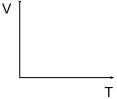
\includegraphics[width=0.35\textwidth]{\figpath/Model1_VTaxes}}
		}
			\centerline{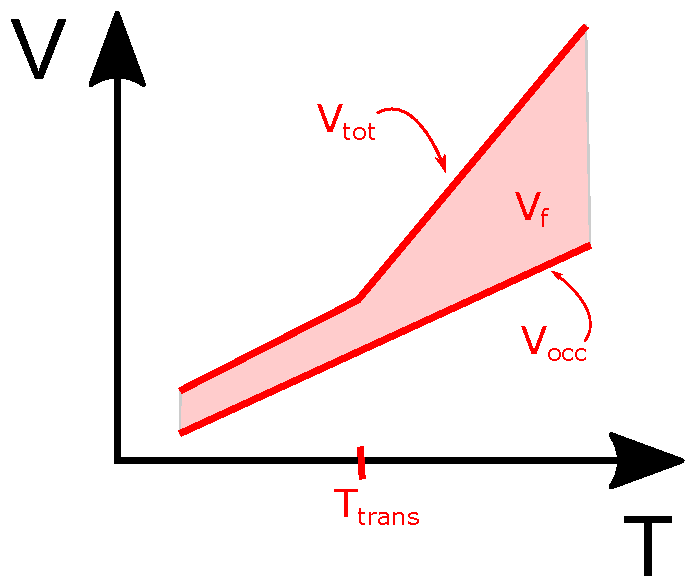
\includegraphics[width=0.35\textwidth]{\figpath/Model1_VTaxes_ctq5}}
			
			%Note: this question is typically pretty hard for students.
		\end{solution}
		
	\question Which type of materials properties (liquid-like or solid-like) do you expect to observe in each of the following limits?  Briefly indicate your group's reasoning. \label{\labelbase:ctq:properties}
	
		\begin{enumerate}
			\item Temperatures far above the transition temperature:
			
				\begin{solution}[0.5in]{}
					At temperatures far above the transition temperature, the polymer is dynamic, has plenty of room to move around, and should be able to flow, so should be liquid-like.
				\end{solution}
			
			\item Temperatures far below the transition temperature:
			
				\begin{solution}[0.5in]{}
					At temperatures far below the transition temperature, the polymer chains are essentially trapped and cannot flow or rearrange, so the material should be solid-like.
				\end{solution}
			
		\end{enumerate}
		
	\question The temperature you explored in CTQs \ref{\labelbase:ctq:traptemp} and \ref{\labelbase:ctq:properties} is known as the \emph{glass transition temperature}, or $T_g$.  A well-known polymer chemistry book states,
	
		\emph{``The value of $T_g$ is the single most important characteristic in choosing a polymer for a given application.''}
		
		Why do you think the authors make this claim?  Explain your group's reasoning in 1-2 complete sentences.
			
				\begin{solution}[1.75in]{}
				
					The polymer's $T_g$ determines whether the polymer will be liquid-like or solid-like at the application temperature.  If you want your polymer to be flexible or liquid-like, you need to choose a polymer whose $T_g$ is well below the temperature at which it will be used.  On the other hand, if you want your polymer to be rigid or solid-like, you need to choose a polymer whose $T_g$ is well above the temperature at which it will be used.
					
					A useful example is the use of poly(lactide) as a material for making plastic cups.  PLA's $T_g$ is approximately 60~$^\circ$C.  If you put a cold drink in a PLA cup, it will be just fine - the temperature of the drink is below the $T_g$ of the cup material so the cup will be just fine and hold its shape.  If you put a hot drink in a PLA cup, however, watch out - a hot drink that is served at 70 to 80~$^\circ$C will cause the cup to soften and ``melt'' because it will take the cup material above its $T_g$.
					
					Note: the quoted statement comes from chapter 12 of \emph{Polymer Chemistry} by Hiemenz \& Lodge.
				
				\end{solution}
	
\end{ctqs}

\begin{model}[The Role of Chain Ends]
\label{\labelbase:mdl:chainends}
	
	Schematics of two polymer samples are shown below:
	
	\vspace{6pt}
	\centerline{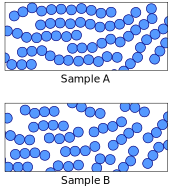
\includegraphics[width=0.4\textwidth]{\figpath/Model2_Mw}}
	
	For the purposes of this Model, you may assume that both samples are made from the same monomer, and differ only in their molecular weight.
	
\end{model}

\begin{ctqs}

	\question Based on the schematics in the model...
		\begin{enumerate}
			\item ... which sample has the higher molecular weight?
				
				\begin{solution}[0.25in]{}
					Sample A
				\end{solution}
				
			\item ... which sample has the higher free volume?
				
				\begin{solution}[0.25in]{}
					Sample B
				\end{solution}
				
		\end{enumerate}
		
	\question Based on your observations of the model, critique or defend the following statement in 1-2 complete sentences:
	
		\emph{``Decreasing the molecular weight of a polymer typically decreases the amount of free volume in a sample of that polymer.''}
		
		\begin{solution}[1.75in]{}
			This statement is generally false.  As shown in the model, the polymer with the \emph{lower} molecular weight appears to have more free volume, not the polymer with the higher molecular weight.  Although students are not asked to propose a reason for this in the question, this relationship occurs because the covalent bonds within the polymer are shorter than the intermolecular distances; since chain ends have fewer covalent bonds to other monomers, there will be more space around them than there is around repeat units in the middles of the chains.
		\end{solution}
	
	\question Suppose the two samples shown in Model \ref{\labelbase:mdl:chainends} start at the same temperature and are then slowly cooled.  Which one do you expect to ``get stuck'' and be unable to further rearrange first? 
	
		\begin{solution}[0.75in]{}
			Sample A has less free volume to start with, so sample A will probably ``run out'' of free volume at a higher temperature than sample B will.
			
			Alternatively, students may reason that the shorter chains in sample B are likely to have an easier time finding their way through small spaces, so should remain mobile to lower temperatures.
		\end{solution}
		
	\question Based on your answer to the previous question, which sample do you expect to have a higher $T_g$?
		 \label{\labelbase:ctq:TgMnPredict}
	
		\begin{solution}[0.75in]{}
			The glass transition occurs when the material no longer has enough free volume for the polymer chains to rearrange.  Since sample A will likely hit this point at a higher temperature than sample B, sample A will have the higher glass transition temperature.
		\end{solution}
	
\end{ctqs}

\begin{infobox}

	The molecular weight dependence of the glass transition temperature is typically found to obey
	\begin{equation*}
		T_g = T_{g,\infty} - \frac{A}{M_n}\label{\labelbase:eqn:Mn}
	\end{equation*}
	where $T_{g,\infty}$ and $A$ are experimentally-determined constants.
\end{infobox}

\begin{ctqs}
	\question Is this equation consistent with your prediction from CTQ \ref{\labelbase:ctq:TgMnPredict}? Why or why not?
	
		\begin{solution}[1in]{}
			Yes, it should be - increasing $M_n$ makes the fraction $A/M_n$ smaller, and the $-A/M_n$ term is thus less negative/reduces the $T_g$ less than when $M_n$ is bigger.
		\end{solution}
	
	\question As $M_n\to\infty$, what happens to the value of $T_g$?  Briefly explain how your group would interpret the $T_{g,\infty}$ term in the equation presented in the information box.
	
		\begin{solution}[1in]{}
			As $M_n\to\infty$, the $A/M_n$ term goes to zero, so $T_g$ approaches $T_{g,\infty}$.  $T_{g,\infty}$ is thus the infinite molecular weight limit of the glass transition temperature.
		\end{solution}
	
\end{ctqs}

\clearpage
\begin{model}[Molecular Determinants of $T_g$]
	\label{\labelbase:mdl:Tgdeterminants}

	Several series of polymers, and their glass transition temperatures, are shown below:
	
	\centerline{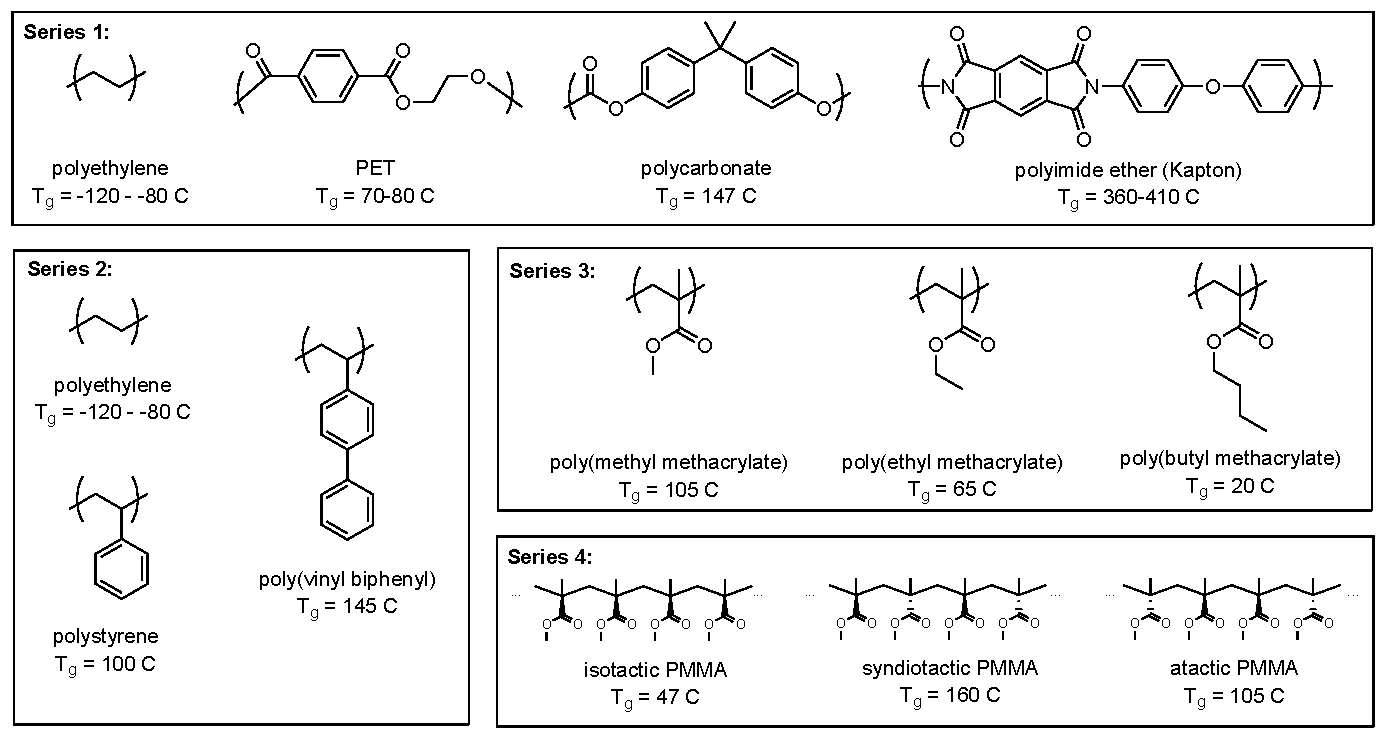
\includegraphics[width=\textwidth]{\figpath/Model3}}
	%Note: values for PMMA are from 10.1002/pol.1966.160040204; other references report a lower Tg for syndiotactic, but the characterization of the tacticity is not always convincing.
	
\end{model}

\begin{ctqs}
	
	\question Based on the structures shown in series 1, what can you infer about how the \emph{stiffness of a polymer's backbone} affects its glass transition temperature?  Propose a reason for the observed trend.
	
		\begin{solution}[0.75in]{}
			Increasing the stiffness of the backbone typically increases the $T_g$ of the polymer.  This is because stiffer polymers have a harder time rearranging and will become trapped/frozen in place at higher temperatures than more flexible polymers will.
		\end{solution}
	

	\question Based on the structures shown in series 2, what can you infer about how the \emph{bulkiness of a polymer's sidechains} affects its glass transition temperature?  Propose a reason for the observed trend.
	
		\begin{solution}[0.75in]{}
			Increasing the bulkiness of a polymer's sidechain typically also increases the polymer's $T_g$.  Again, bulkier sidechains need more space to be able to rearrange, so polymers with bulky sidechains will become trapped/frozen in place at higher temperatures than polymers with smaller or more flexible sidechains.
		\end{solution}
	
	\question Based on the structures shown in series 3, what can you infer about how the \emph{flexibility of a polymer's sidechains} affects its glass transition temperature?  Propose a reason for the observed trend.
	
		\begin{solution}[1in]{}
			Adding small, flexible sidechains to a polymer typically \emph{decreases} its $T_g$.  This is for much the same reason as chain ends do, as discussed in Model 2 - the small, flexible sidechains essentially act as impurities that increase the free volume of the material.  (Note, however, that long, aliphatic sidechains can reverse this trend once they become long enough to crystalize).
		\end{solution}
		
	\question Based on the structures shown in series 4, what can you infer about how the \emph{stereochemistry of a polymer} affects its glass transition temperature?  Propose a reason for the observed trend.
	
		\begin{solution}[1in]{}
			Typically, for alkyl acrylates, $T_{g,isotactic}<T_{g,atactic}<T_{g,syndiotactic}$.  The reason for this behavior is complicated, but it is thought to arise from changes to the steric barriers for rotation that result in effective stiffening of the chains (see e.g. DOIs 10.1021/ma990888f and 10.1021/acs.macromol.8b01099, which discuss this effect for polypropylene).  Students probably will not get this point, but should have an interesting discussion!
			
			Polymers with smaller sidechains but very \emph{regular} patterns of stereocenters (e.g. isotactic and syndiotactic samples of polymers like polypropylene) may also have an increased ability to partially crystallize, which can also affect $T_g$.
		\end{solution}
	
	\question In a short paragraph, summarize what you have learned about the key features that determine a polymer's glass transition temperature.
	
		\begin{solution}[2in]{}
			Generally speaking, features of the polymer that make it harder for the polymer to move easily, such as stiffness and bulkiness, will increase the $T_g$ of the polymer.  Features of the polymer that increase the free volume of the system, on the other hand, such as low molecular weights (i.e. lots of chain ends), flexible sidechains, and small-molecule plasticizers, will make it easier for the system to rearrange even at lower temperatures and will lower $T_g$.
		\end{solution}
	
\end{ctqs}

\begin{exercises}

	\exercise Experimentally, it is often found that cooling a sample quickly results in a higher $T_g$ than cooling the same sample slowly.  Propose a reason why this might be true, based on your understanding of how the timescale for rearrangement of the polymer chains depends on temperature.
	
		\begin{solution}{}
		
			The key idea in this question is that the glass transition is fundamentally a \emph{kinetic} effect.  The glass transition occurs when the polymers are no longer able to move around to find more favorable configurations.  Because motions of polymer chains typically slow down at lower temperatures, a polymer will need a longer time to find these more favorable configurations as the temperature decreases.
			
			The result is that when a polymer is cooled very slowly, it has more time to find favorable configurations even at lower temperatures, and so it is able to keep rearranging at lower temperatures; when a polymer is cooled very quickly, on the other hand, it may not have enough time to find favorable configurations at some of the higher temperatures before the temperature is dropped again, and its configuration will become trapped at a higher temperature, giving rise to a higher $T_g$.
		
		\end{solution}
	
	\exercise For polystyrene, the value of $A$ in the equation on page \pageref{\labelbase:eqn:Mn} is approximately $10^5$~K~g/mol.  Above what molecular weight would you expect the measured $T_g$ to be within 10~$^\circ$C of the infinite molecular weight limit?
	
		\begin{solution}{}
			We want to find the value of $M_n$ that gives $T_{g,\infty} - T_g=10\,{}^\circ$C.  To do so, first rearrange the equation as follows:
			\begin{align*}
				T_{g,\infty} - T_g = \frac{A}{M_n}\\
				M_n = \frac{A}{T_{g,\infty} - T_g}
			\end{align*}
			Then, substituting in the given values, we find
			\begin{align*}
				M_n &= \frac{10^5\text{ K g/mol}}{10\text{ K}}\\
					&= 10^4\text{ g/mol}
			\end{align*}
			Thus, the $T_g$ will be within 10~$^\circ$C of the infinite molecular weight limit when the molecular weight is greater than 10~kg/mol.
		\end{solution}
	
	%\exercise In this activity, you looked at the VFT equation for the temperature dependence of the viscosity of a polymer.  This equation referenced the Vogel temperature, $T_0$, along with two other fittigng parameters, $A$ and $B$.	In many practical applications, however, it is more useful to instead express how the viscosity changes relative to a reference temperature.  After some math, it is possible to show that
	%\begin{equation*}
	%	\log\left(\frac{\eta}{\eta_r}\right) = -\frac{C_1(T-T_r)}{C_2 + (T-T_r)}
	%\end{equation*}
	%where $\eta_r$ is the viscosity at reference temperature $T_r$ and $C_1$ and $C_2$ are experimentally-determined parameters.  This equation is called the \emph{Williams-Landel-Ferry \emph{(or WLF)} equation.}
	
	%\exercise It is possible to show that the viscosity of a polymer melt scales with molecular weight as
	%	\begin{equation*}
	%		\eta \sim M^{3.4}
	%	\end{equation*}
		
	%	\dots
	
	%\exercise walk students through deriving/justifying the molecular weight dependence of $T_g$ a la the treatment in Young and Lovell section 16.3
	
	\exercise Empirically, it is found that the $T_g$'s of polymer blends and copolymers typically obey the Fox equation, which for a two-component blend can be expressed as\footnote{A more general form of this equation, for blends containing more than two components, is $\frac{1}{T_{g,mix}} = \sum_i \frac{w_i}{T_{g,i}}$, where $w_i$ is the weight fraction of component $i$ and $T_{g,i}$ is its $T_g$.}
		\begin{equation*}
			\frac{1}{T_{g,mix}} = \frac{w_A}{T_{g,A}} + \frac{w_B}{T_{g,B}}
		\end{equation*}
		where $w_A$ is the weight fraction of polymer A, $T_{g,A}$ is the $T_g$ of component A, and $w_B$ and $T_{g,B}$ are similarly the weight fraction and $T_g$ of component B.
		
		Suppose you prepare a blend of 1~g of polystyrene ($T_g = 100$~$^\circ$C) and 1~g of poly(\emph{p}-phenylene oxide) ($T_g = 215$~$^\circ$C).  Based on the Fox equation, given above, what do you expect the $T_g$ of the resulting blend to be?
		% the data on this page: http://polymerdatabase.com/polymer%20physics/Fox.html for butadienes with different cis/trans/vinyl fractions would also make a great exam question!
		
		\begin{solution}{}
			Because we have equal masses of both polymers, $w_{PS} = w_{PPO} = 0.5$.  From there, we can simply plug into the given equation (making sure to convert temperatures to Kelvin!) to obtain
			\begin{align*}
				\frac{1}{T_{g,mix}} &= \frac{0.5}{(100+273)\text{ K}} + \frac{0.5}{(215+273)\text{ K}}\\
					\, &= 0.002365\text{ K}^{-1}\\
				T_{g,mix} &= 423\text{ K}\\
				&= 149\text{ }^\circ\text{C}
			\end{align*}
		\end{solution}
	
\end{exercises}


%\begin{problems}
%
%	\problem First exercise
%	\problem Second exercise
%	
%\end{problems}


	
\end{activity}